\chapter{Inverse Kinematics}
\section{Important}
Read the entire lab before starting and especially the ``Grading" section so you are aware of all due dates and requirements associated with the lab.  Hopefully you are reading this well before your lab section meets as given the compressed schedule, it is very important that you arrive at lab well prepared.  This semester, the more you do prior to your lab session, the more you will get out of the short time you have with the TA.
\section{Objectives}
The purpose of this lab is to derive and implement a solution to the inverse kinematics problem for the UR3e robot.  In this lab we will:
\begin{itemize}
	\item Derive elbow-up inverse kinematic equations for the UR3e
	\item Write a Python function that moves the UR3e to a point in space specified by the user.
\end{itemize}

\section{Reference}
Chapter 6 of \textit{Modern Robotics} provides multiple examples of inverse kinematics solutions.

\section{Tasks}
\subsection{Solution Derivation}
\textbf{Make sure to read through this entire lab before you start deriving your solution.  There are some
needed details not covered in this section.}


Given a desired end-effector position in space $(x_{grip},y_{grip},z_{grip})$ and orientation $\left\{\theta_{yaw},\theta_{pitch}(fixed),
\theta_{roll}(fixed)\right\}$, write six mathematical expressions 
that yield values for each of the joint angles. For the UR3e robot, there are many solutions to the inverse kinematics
problem.  We will implement only one of the \textit{elbow-up} solutions.

\begin{itemize}
\item In the inverse kinematics problems you have examined in class (for 6 DOF arms with spherical wrists), usually the first step is to solve
for the coordinates of the wrist center.  The UR3e does not technically have a spherical wrist center but we will define the wrist center as $z_{cen}$
which equals the same desired z value of the suction cup and $x_{cen}$, $y_{cen}$ are the coordinates of $\theta_6$'s z axis.
In addition, to make the derivation manageable,
add that $\theta_5$ will always be $-90^{\circ}$ and $\theta_4$ is set such that link 7 and link 9 are always parallel to the world x,y plane.   
\begin{figure}[tbp]
	\centering
		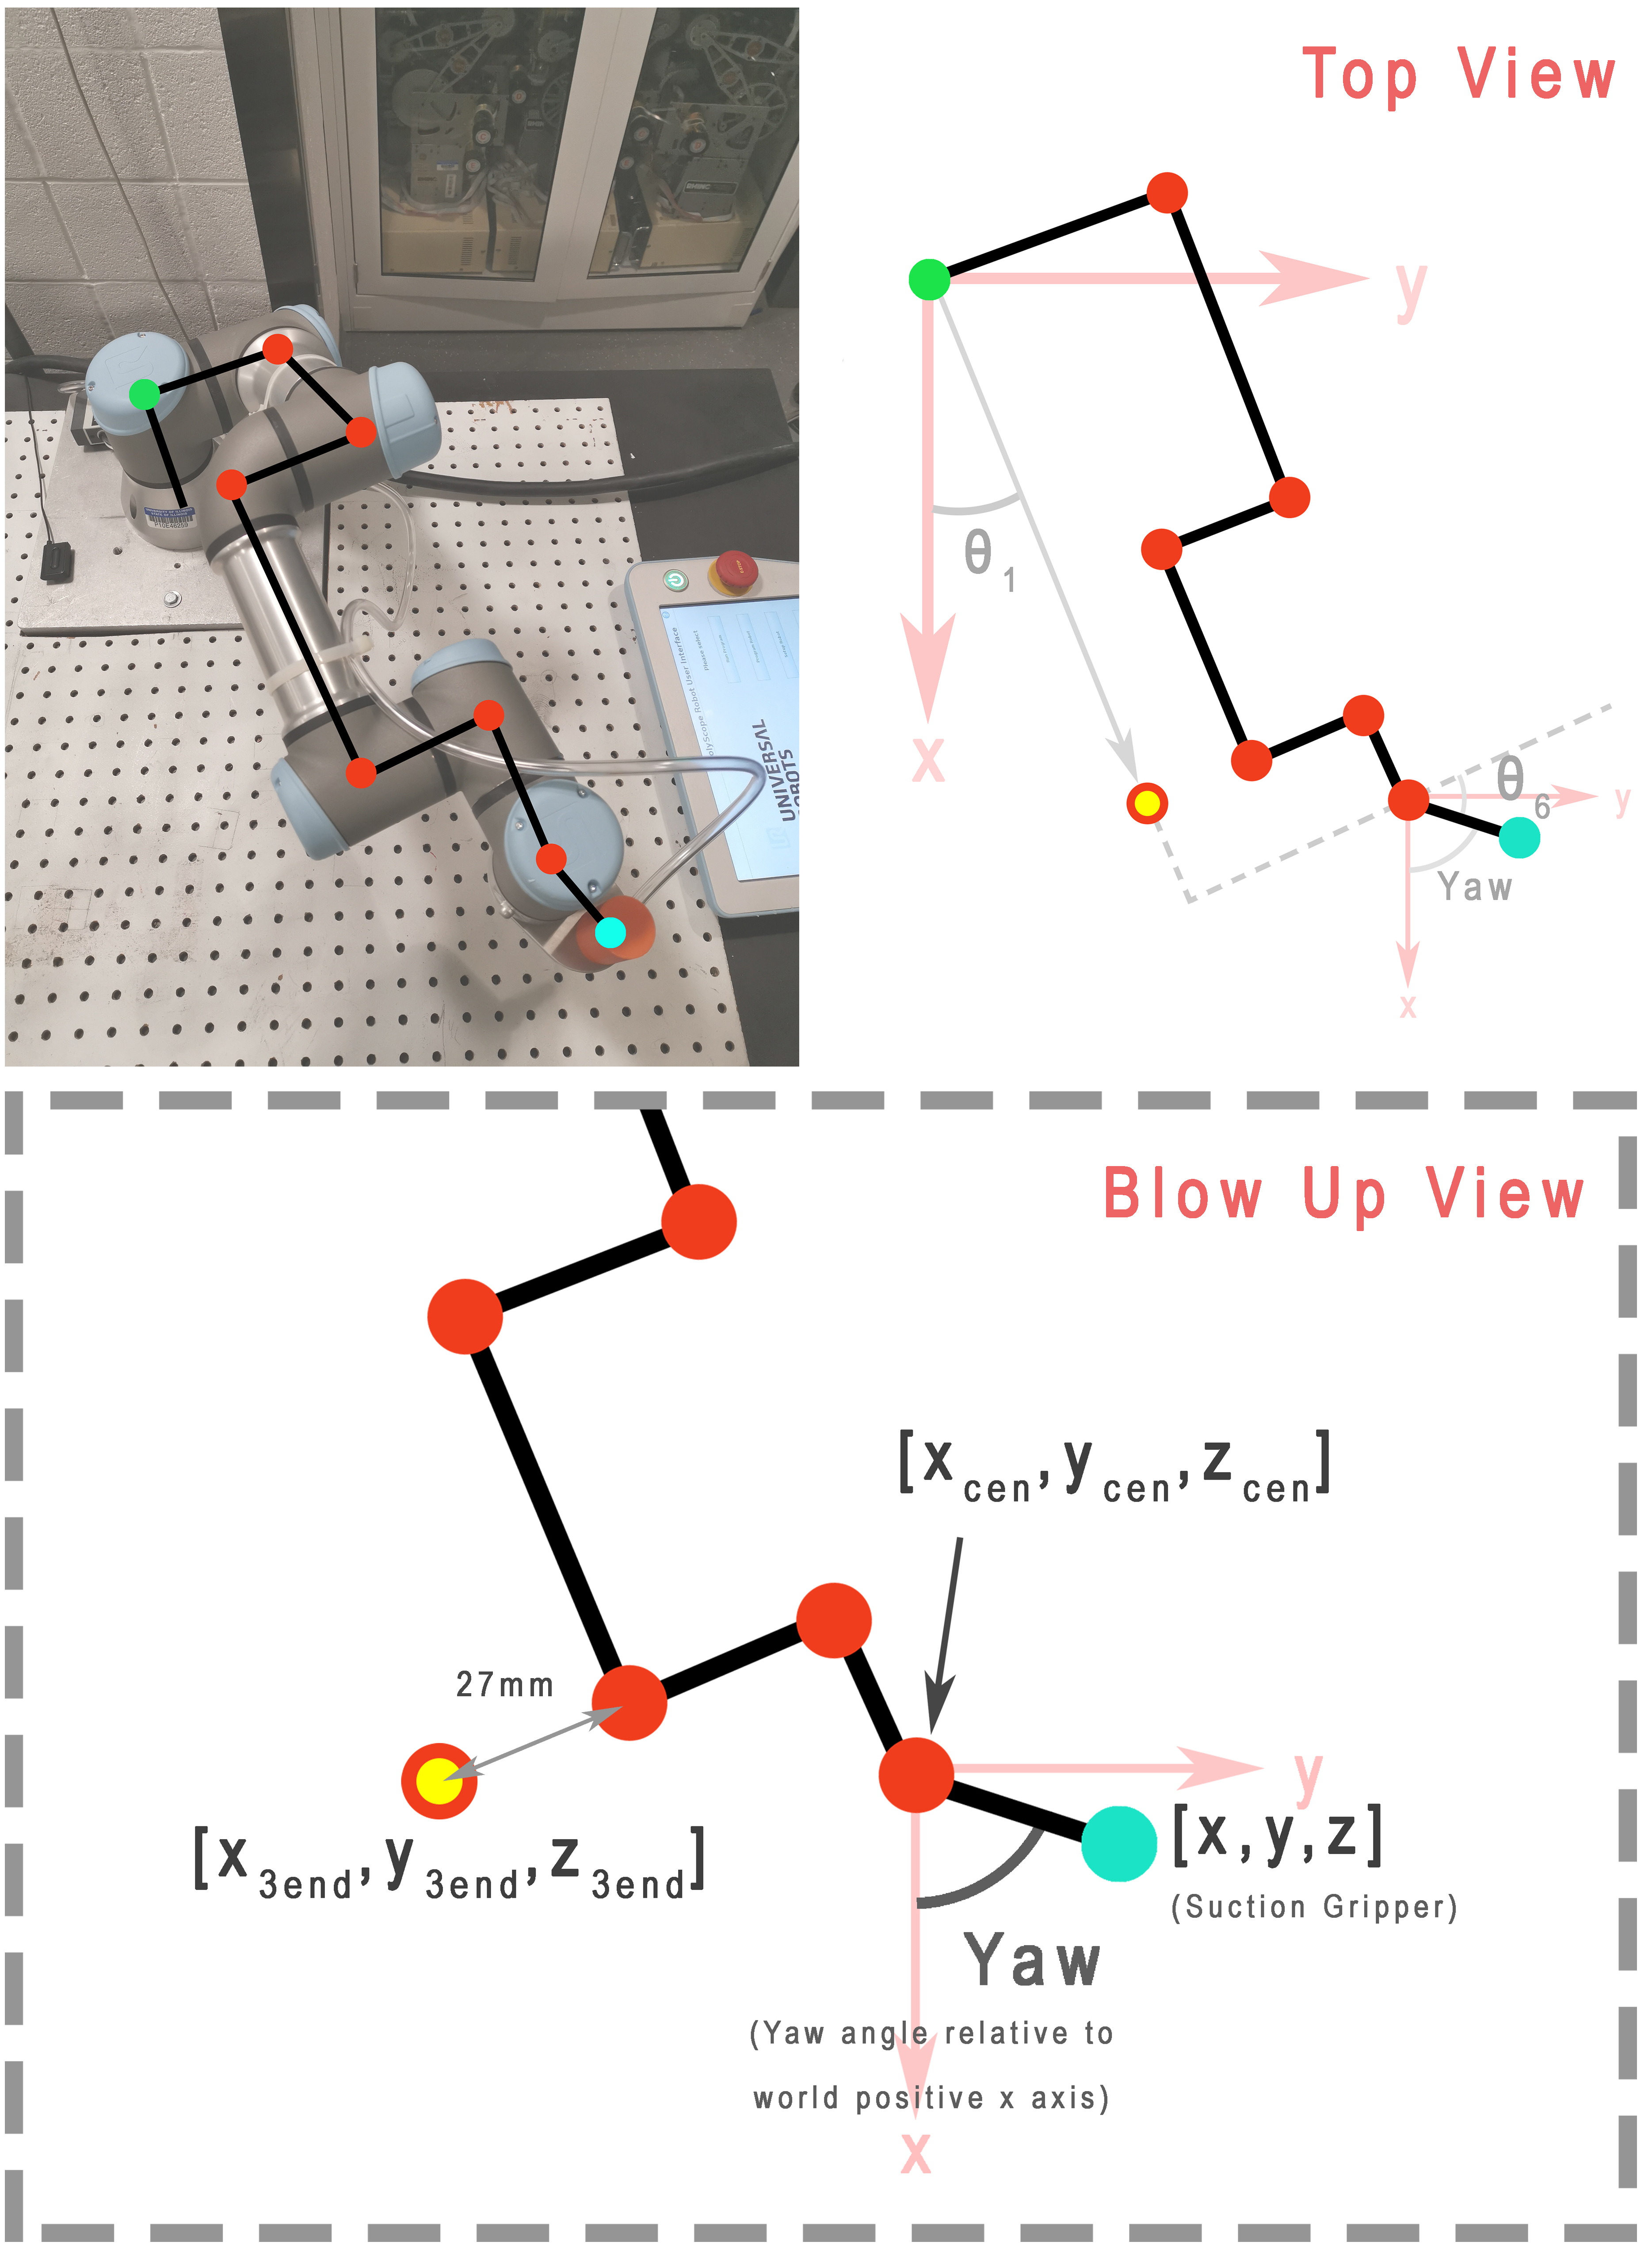
\includegraphics[scale=0.127]{image/lab5_ur3_pre4.jpg}
	\caption{\figlbl{TopView} Top View Stick Pictorial of UR3e. Note that the coordinate frames are in the same direction
	as the World Frame but not at the World frame's origin.  One origin is along the center of joint 1 and the second
	is along the center of joint 6.}
\end{figure}

\begin{figure}[tbp]
	\centering
		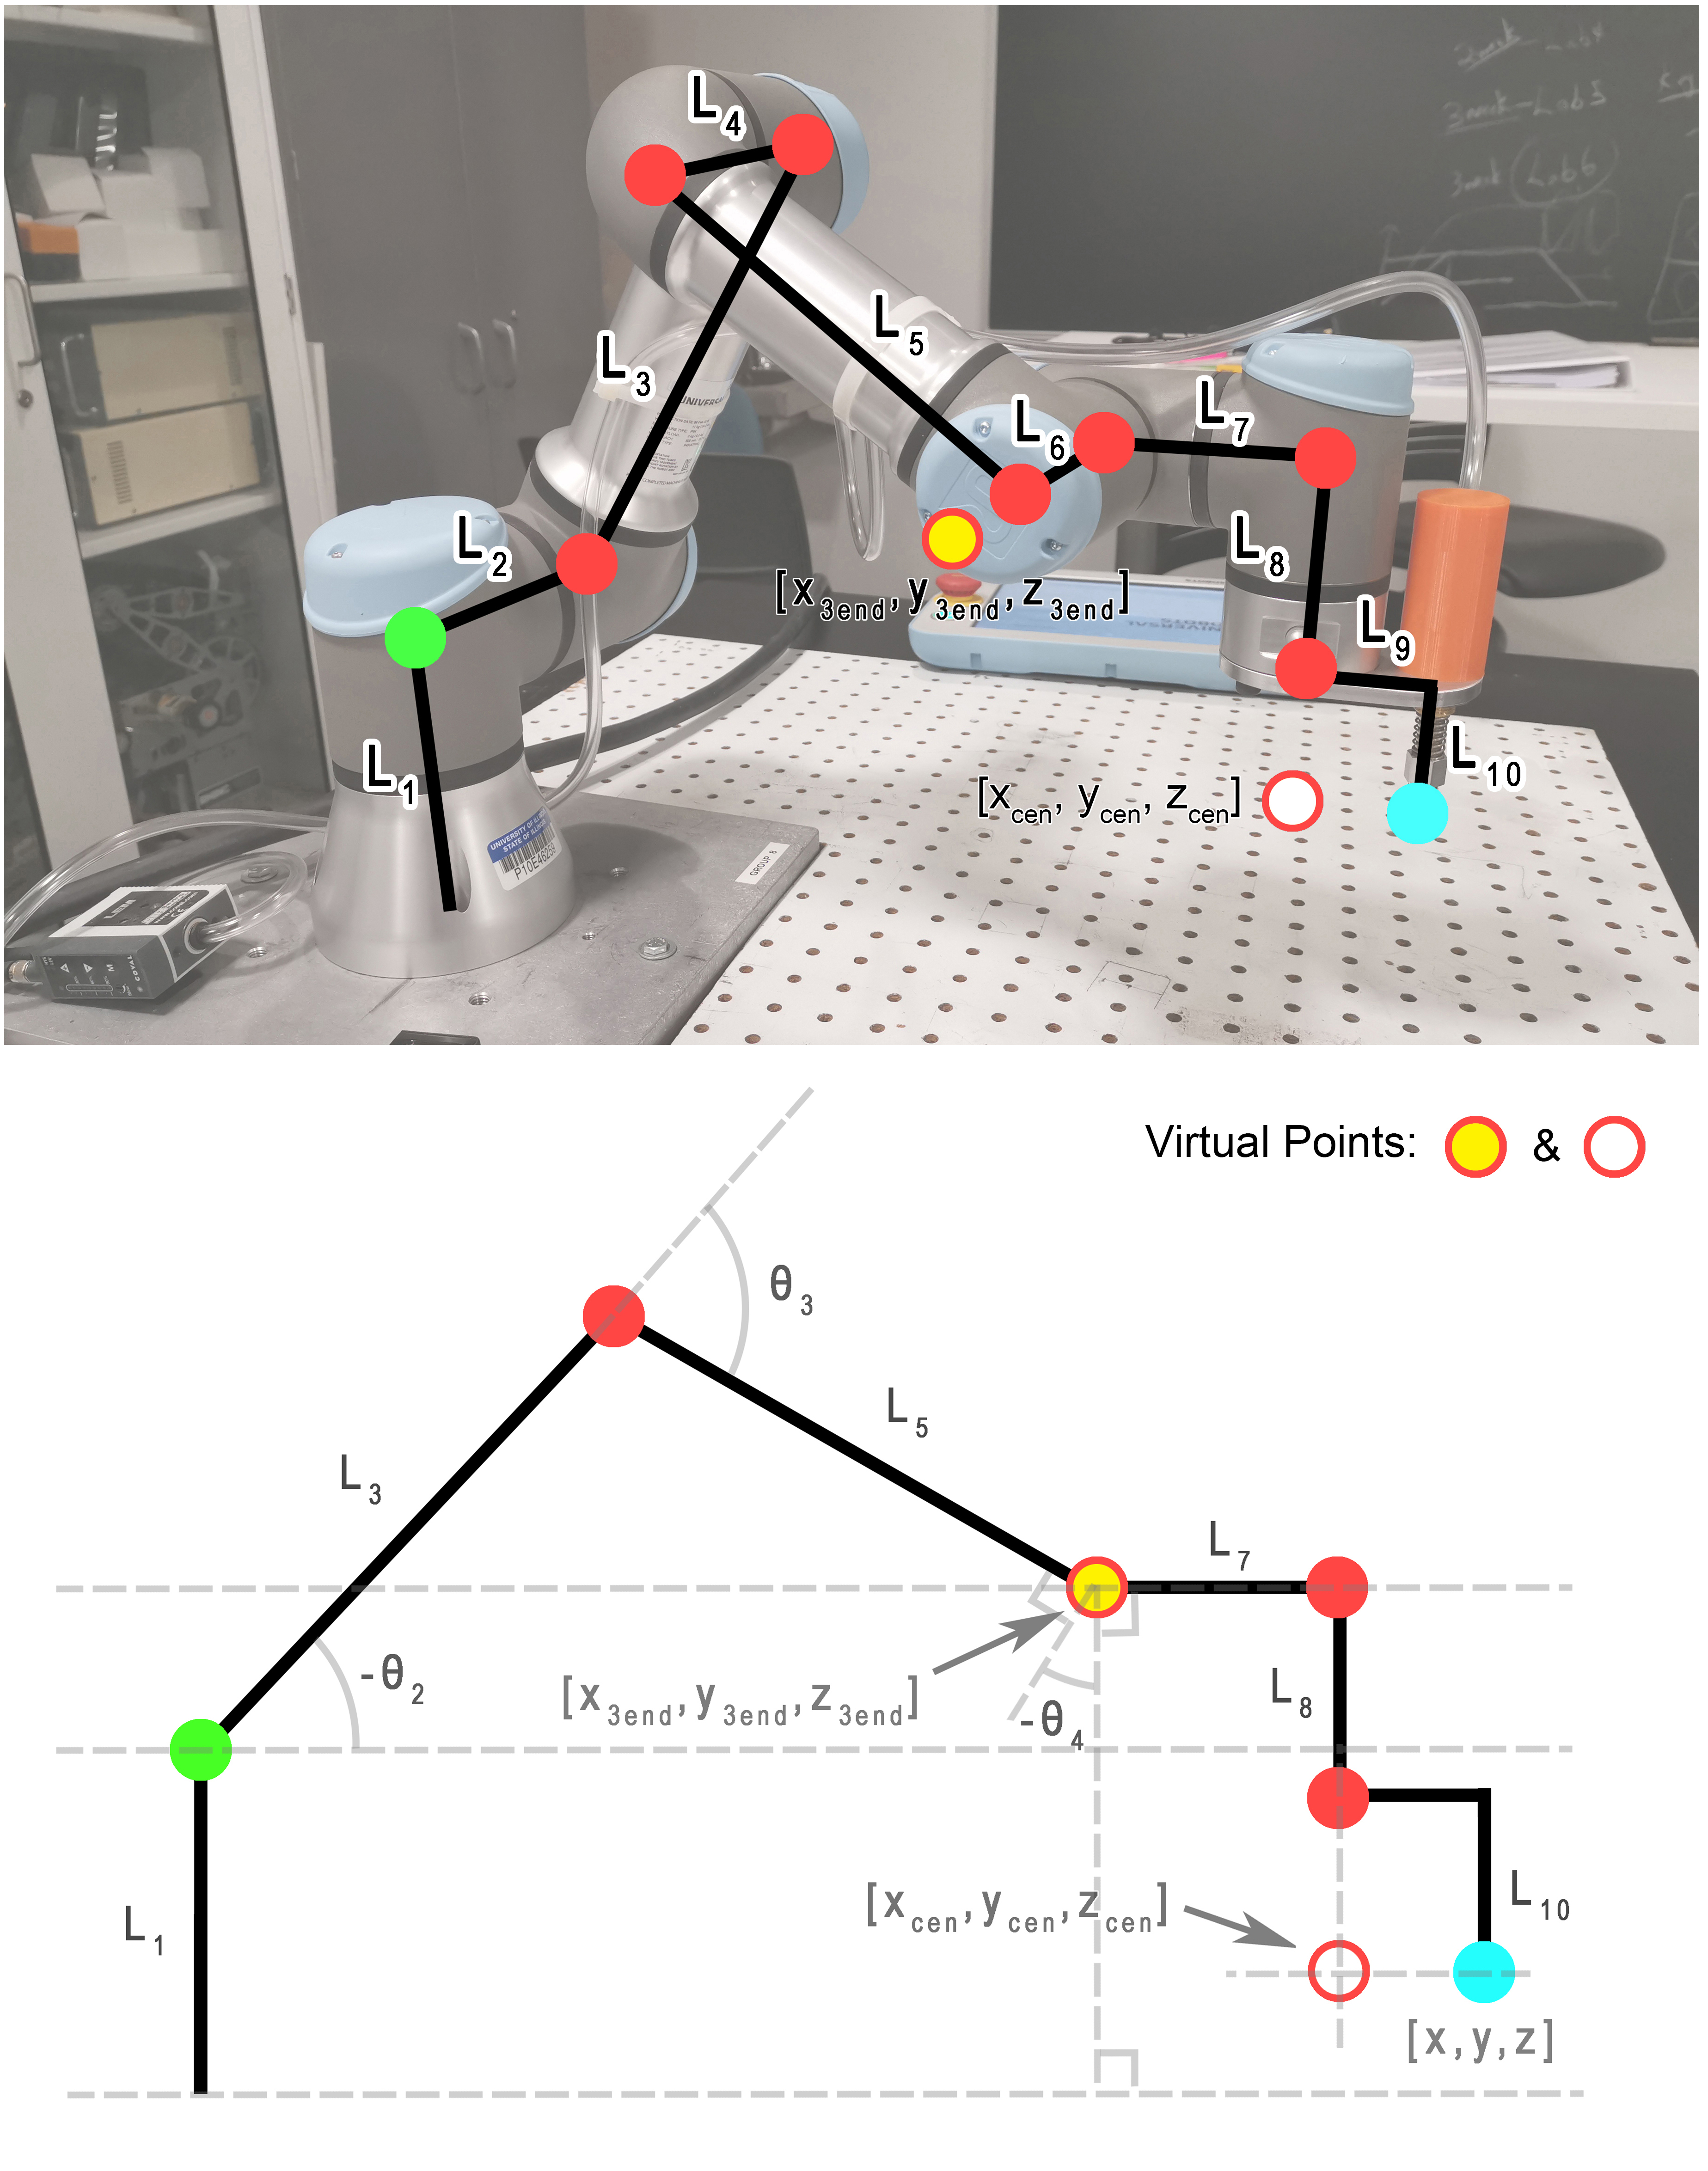
\includegraphics[scale=0.125]{image/lab5_ur3_side3_1_old.jpg}
	\caption{\figlbl{SideView} Side View Stick Pictorial of UR3e.}
\end{figure}

\item Solve the inverse kinematics problem in the following order:
\begin{enumerate}
	\item $x_{cen}$, $y_{cen}$, $z_{cen}$, given yaw desired in the world frame and the desired x,y,z of the suction cup. The suction cup aluminum
plate (link 9) has a length of 0.0535 meters from the center line of the suction cup to the center line of joint 6. Remember that this
aluminum plate should always be parallel to the world's x,y plane.  See \figref{SideView}.	
	\item $\theta_1$, by drawing a top down picture of the UR3e, \figref{TopView}, and using $x_{cen}$, $y_{cen}$, $z_{cen}$ that you just calculated.
	\item $\theta_6$, which is a function of $\theta_1$ and yaw desired.  Remember that when $\theta_6$ is equal to zero the suction cup aluminum plate
is parallel to link 4 and link 6.
  	\item $x_{3end}$, $y_{3end}$, $z_{3end}$ is a point off of the UR3e but lies along the link 6 axis, \figref{TopView}.  For example if $\theta_1 = 0^{\circ}$ then $y_{3end} = 0$.
If $\theta_1 = 90^{\circ}$ then $x_{3end} = 0$.  First use the top down view of the UR3e to find $x_{3end}$, $y_{3end}$.  One way is to choose an appropriate
coordinate frame at $x_{cen}$, $y_{cen}$ and find the translation matrix that rotates and translates that coordinate frame to the base frame.  
Then find the vector in the coordinate frame you chose at $x_{cen}$, $y_{cen}$ that points from $x_{cen}$, $y_{cen}$ to $x_{3end}$, $y_{3end}$.
Simply multiply this vector by your translation matrix to find the world coordinates at $x_{3end}$, $y_{3end}$.  For $z_{3end}$ create a view of
the UR3e, \figref{SideView}, that is a projection of the robot onto a plane perpendicular to the x,y world frame and rotated by $\theta_1$ about
the base frame.  Call this the side view.  Looking at this side view you will see that $z_{3end}$ is $z_{cen}$ offset by a constant.    
	\item $\theta_2$, $\theta_3$ and $\theta_4$, by using the same side view drawing just drawn above to find $z_{3end}$, \figref{SideView}.
Now that $x_{3end}$, $y_{3end}$, $z_{3end}$ have
been found use sine, cosine and the cosine rule to solve for partial angles that make up $\theta_2$, $\theta_3$ and $\theta_4$.  Hint:  In this side view, a parallel to the base construction line through joint 2
and a parallel to the base construction line through joint 4 are helpful in finding the needed partial angles.       		
\end{enumerate}
\end{itemize}

\subsection{Implementation}
Implement the inverse kinematics solution by writing a Python function to receive world frame coordinates $(x_{Wgrip},y_{Wgrip},z_{Wgrip},yaw_{Wgrip})$, compute the desired
joint variables $\left\{\theta_1,\theta_2,\theta_3,\theta_4,\theta_5,\theta_6\right\}$, and command the UR3e to move to that pose
using functions written in Lab4.

\section{Procedure}
\begin{itemize}
	\item Copy \textbf{lab5pkg\_ik} to your workspace.  You will notice that there are three .py files.  
\textbf{lab5\_exec.py}, \textbf{lab5\_func.py} and \textbf{lab5\_header.py}.  The \textbf{lab5\_func.py} file again will be compiled into a library so that future labs can easily call the inverse kinematic
function.  Like Lab 4, most of the needed code is given to you in \textbf{lab5\_exec.py}.  Your main job will be to add all the inverse kinematic equations to
\textbf{lab5\_func.py}. Please refer to the intermediate steps below to perform the inverse kinematic calculations.  If you look
at \textbf{lab5\_header.py} it includes \textbf{lab5\_header.py}.  This allows you to call the functions you created in \textbf{lab5\_func.py}.

    \item Once your code is finished, run it using ``\textbf{rosrun lab5pkg\_ik lab5\_exec.py [x] [y] [z] [yaw(degrees)]}" - e.g. ``\textbf{rosrun lab5pkg\_ik lab5\_exec.py 0.1 0.1 0.15 90}".  Remember to run drivers that in another command prompts at first. 

    \item For in-person students, you should measure the x,y,z position of the end-effector using the provided ruler and square.  For students using the simulation, it is not possible to measure this way, so we must use another method.  A simple way is to use some of the ROS commands we learned before: ``\textbf{rostopic echo /gripper/position -n 1}".  These values are being calculated differently and so there will be small differences between this value and your calculations.
    
    \item You should verify that your code works by selecting a variety of poses that will test the full range of motion.  Your TA will not be providing you test points.

	\item In your code (This is repeating the derivation steps above):
\begin{enumerate}	
	\item Establish the world coordinate frame (frame $w$) centered at the corner of the UR3e's base shown in \figref{frames}.
The $x_w$ and $y_w$ plane should correspond to the surface of the table, with the $x_w$ axis parallel to the sides of the
table and the $y_w$ axis parallel to the front and back edges of the table.  Axis $z_w$ should be normal to the table surface,
with up being the positive $z_w$ direction and the surface of the table corresponding to $z_w=0$.\\
We will solve the inverse kinematics problem in the base frame (frame 0), so we will immediately convert the coordinates entered by
the user to base frame coordinates.  Write three equations relating coordinates $(x_{Wgrip},y_{Wgrip},z_{Wgrip})$ in the world frame to coordinates
$(x_{grip},y_{grip},z_{grip})$ in the base frame of the UR3e.  
  \begin{eqnarray*}
	x_{grip}(x_{Wgrip},y_{Wgrip},z_{Wgrip}) =\\
	y_{grip}(x_{Wgrip},y_{Wgrip},z_{Wgrip}) =\\
	z_{grip}(x_{Wgrip},y_{Wgrip},z_{Wgrip}) =
	\end{eqnarray*}

\begin{figure}[h]
	\centering
		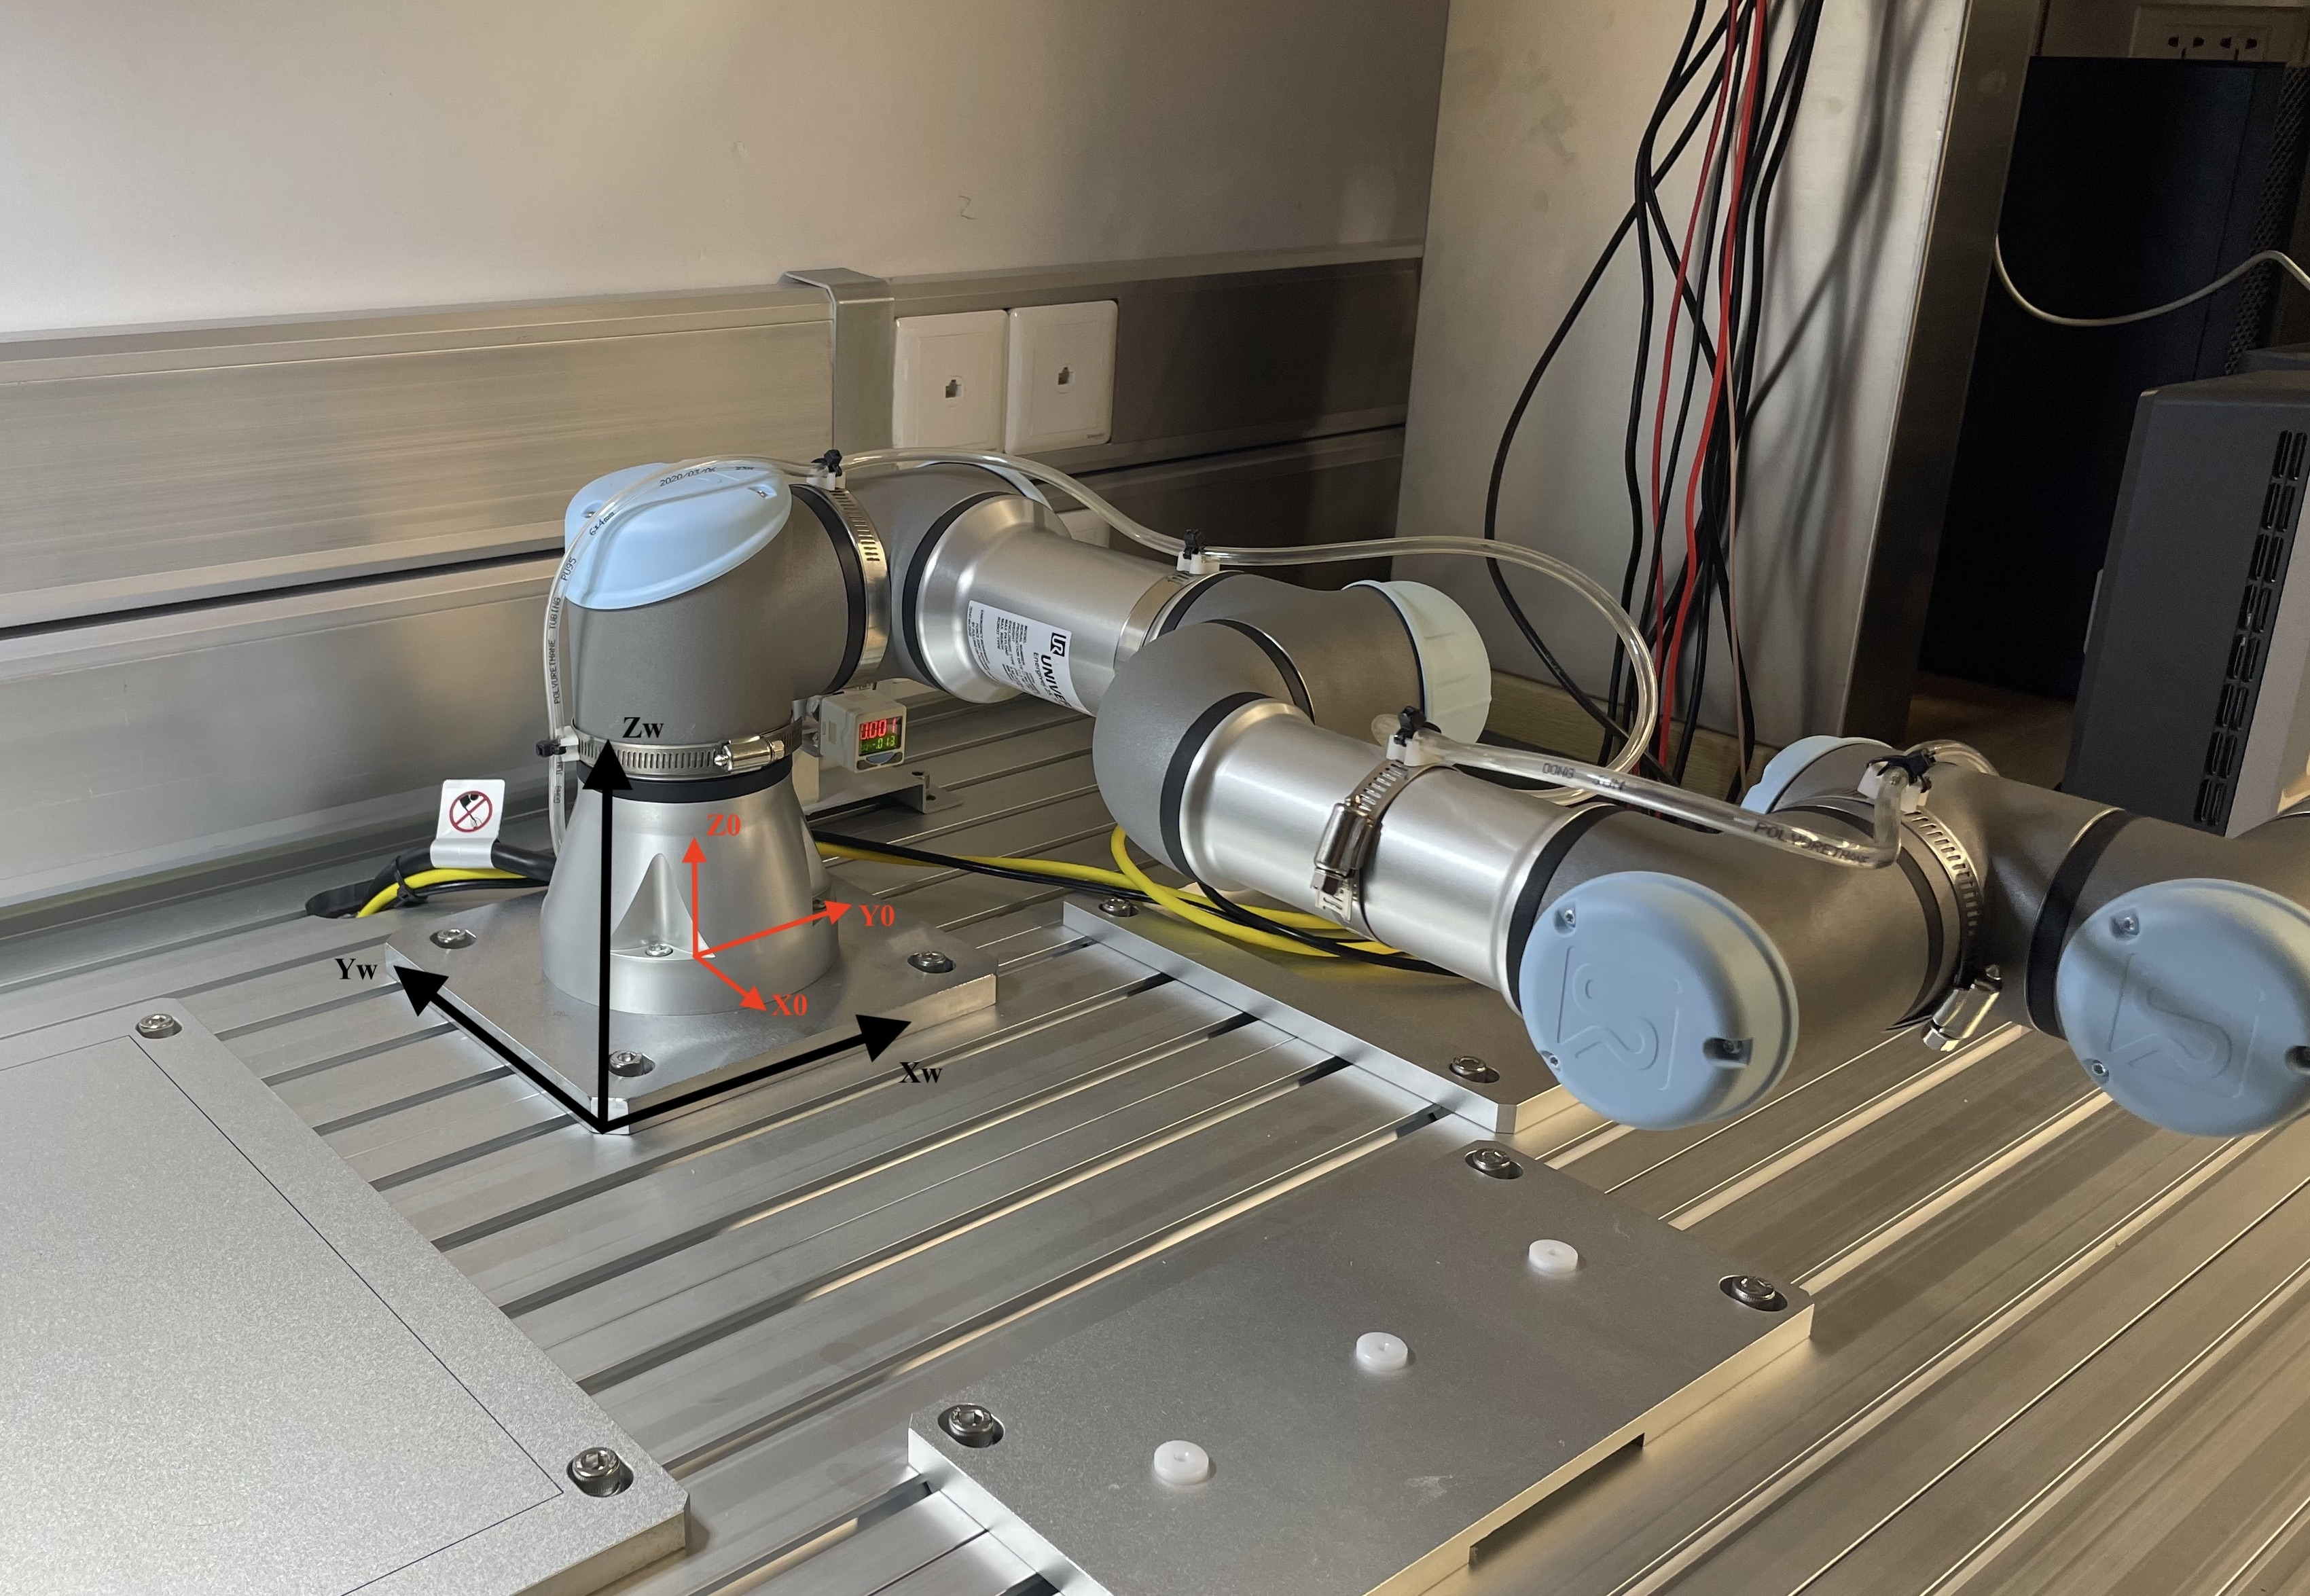
\includegraphics[scale=0.75]{image/lab5_wf0f_1.jpg}
	\caption{\figlbl{frames} Correct location and orientation of the world frame.}
\end{figure}

\item Given the desired position of the gripper $(x_{grip},y_{grip},z_{grip})$ (in the base frame) and the yaw angle, find wrist's center point $(x_{cen},y_{cen},z_{cen})$.
\begin{eqnarray*}
	x_{cen}(x_{grip},y_{grip},z_{grip},yaw) =\\
	y_{cen}(x_{grip},y_{grip},z_{grip},yaw) =\\
	z_{cen}(x_{grip},y_{grip},z_{grip},yaw) = 
\end{eqnarray*}

\item Given the wrist's center point $(x_{cen},y_{cen},z_{cen})$, write an expression for the waist angle $\theta_1$.  Make sure to use the \textbf{atan2()} 
function instead of \textbf{atan()} because \textbf{atan2()} takes care of the four quadrants the x,y coordinates could be in.  
\begin{equation}
	\theta_1(x_{cen},y_{cen},z_{cen}) = 
\end{equation}
\item Solve for the value of $\theta_6$, given yaw and $\theta_1$.
\begin{equation}
	\theta_6(\theta_1,yaw) = 
\end{equation}
\item Find the projected end point $(x_{3end},y_{3end},z_{3end})$ using $(x_{cen},y_{cen},z_{cen})$ and $\theta_1$.  
\begin{eqnarray*}
	x_{3end}(x_{cen},y_{cen},z_{cen},\theta_1) =\\
	y_{3end}(x_{cen},y_{cen},z_{cen},\theta_1) =\\
	z_{3end}(x_{cen},y_{cen},z_{cen},\theta_1) = 
\end{eqnarray*}

\item Write expressions for $\theta_2$, $\theta_3$ and $\theta_4$ in terms of the end point.  You probably will want to define some intermediate
variables to help you with these calculations.
\begin{eqnarray*}
	\theta_2(x_{3end},y_{3end},z_{3end}) =\\
	\theta_3(x_{3end},y_{3end},z_{3end}) =\\
	\theta_4(x_{3end},y_{3end},z_{3end}) = 
\end{eqnarray*}

\item Now that your code solves for all the joint variables (remember that $\theta_5$ is always $-90^{\circ}$) send these six values to the Lab 4 
function \textbf{lab\_fk()}.  You will need to copy you Lab 4 solution into these functions. Do this simply to check that your inverse kinematic calculations are correct. Double check that the x,y,z point that you asked the robot
to go to is the same value displayed by the forward kinematic equations.

\end{enumerate}	
\end{itemize}	

\newpage

\section{Report}
You should submit a lab report using the guidelines given in the ECE 470: How to Write a Lab Report document.  Please be aware of the following:
\begin{itemize}
    \item \textbf{Lab reports are due with your demo for lab 5!}
    \item Lab reports will be submitted online at \href{https://learn.intl.zju.edu.cn/}{Blackboard}.
\end{itemize}
Your lab report should include the following:
\begin{itemize}
% 	\item Coversheet containing your name name, ``Lab 4'', and the weekday and time your lab section meets (for example, ``Tuesday, 3pm'').
    \item A clearly written derivation of the inverse kinematics solution for each joint variable $\left(\theta_{1},\theta_{2},\theta_{3},\theta_{4},\theta_{5},\theta_{6}\right)$. You \textbf{must} include figures in your derivation. Diagrams should be your own creation and clear and easily read.  Do not use hand drawn figures or annotations.
\item For each test point include:
    \begin{itemize}
        \item The given $\{\left(x_{w_{grip}}, y_{w_{grip}},z_{w_{grip}}\right),\theta_{yaw}\}$
        \item The measured position
        \item The scalar error
    \end{itemize}
\item Include a brief discussion of sources of error.

\end{itemize}

As appendices to your report, include the following:
\begin{itemize}
    \item Your $\textbf{lab5\_func.py}$ code and $\textbf{lab5\_exec.py}$ if it was edited.
\end{itemize}

\section{Demo}
Your TA will require you to run your program twice, each time with a different set of desired position and orientation. Your program should reach the desired position and orientation with almost no error. You will be required to be able to demo on the simulator, even if you choose to demo on the real robot.

\section{Grading}
\begin{itemize}
% \item If you don't show up in the in-person and online labs, you \textbf{automatically lose up to 30 points} unless you have a excused absence. Not seeing this line is not a valid one.
% \item 10 points, by the \textbf{end of the first two hour lab session}, show your TA your equations for finding $x_{cen}$, $y_{cen}$, $z_{cen}$.
% \item 10 points, take home assignment after first two hour lab session, by the \textbf{start of the second two hour lab session}, show your TA your equations for $\left\{\theta_1,\theta_2,\theta_3,\theta_4,\theta_5,\theta_6\right\}$.
% \item 10 points, by the \textbf{end of the second two hour lab session}, show your TA your inverse kinematic equations for $\left\{\theta_1,\theta_2,\theta_3,\theta_4,\theta_5,\theta_6\right\}$ implemented in Python code.  
\item 80 points, successful demonstration.
\item 20 points, individual report.  
\end{itemize}


% \section{Tentative Due Dates - Fall 2020}
% The exact date and time will depend on your lab section and can be found on \href{https://learn.intl.zju.edu.cn/}{Blackboard}.
% \subsection{Group A}
% \begin{itemize}
%     \item Demonstration - Week of November 16
%     \item Report - Week of November 16
% \end{itemize}

% \subsection{Group B}
% \begin{itemize}
%     \item Demonstration - Week of November 30
%     \item Report - Week of November 30
% \end{itemize}